\chapter{Application de la FWI à des données simulées \label{applications}}

p91 potel bruneau en francais: données "d'aspect limité" : il n'est pas possible de tourner autour de l'obstacle. On compense la perte d'info en réalisant les mesures sur plusieurs freq et possibilité de déplacer capteur.

\section{Génération des données observées}

Les données de référence sont générées par la résolution d'un problème direct.
Le signal d'excitation choisi est une fonction de Ricker qui correspond à la dérivée seconde d'une Gaussienne et qui est définie de la manière suivante : 
\begin{equation}
	s(t)=(1-(t-t_{0}f\pi))^2e^{-((t-t_{0})\pi f)^2}\text{.}
\end{equation}
\todo[inline]{Est-ce réaliste ?}

Deux barrettes de 64 éléments sont utilisées en réception et en transmission. La fréquence centrale d'excitation est 2 MHz.



%\section{Discrétisation}

%Les discrétisations spatiales et temporelles sont contraintes par
%2 conditions sur la discrétisation : 
%CFL et ..points par longueur d'onde pour les schéma d'ordre ... et... (en différences finies)

\section{Analyse de résolution spatiale}
En théorie, si l'éclairage est parfait, on est limité en résolution par lambda/2 (cf review virieux ou thèse de romain : "pouvoir de résolution du gradient"). En pratique, tout comme en ray-tomo (cf wiliamson cité dans review virieux), on est très limité par l'éclairage.

Afin de déterminer le pouvoir de résolution du gradient, \cite{sirgue} réalise une analyse en onde plane comme suit. Considérons une onde plane incidente se propageant vers un point diffractant (suivant $\bm{s}$), donnant naissance en ce point à une autre onde plane se propageant suivant $\bm{r}$ (cf figure~\ref{}).\todo[inline]{pourquoi pas vers le récep ? i e Sirgue 2004 p.3 : pourquoi tous ces conjugués ?}

\begin{equation}
	k= \frac{\omega}{c} 2 \cos\left( \frac{\theta}{2}\right)
\end{equation}

La résolution est donc maximale quand $\theta=0$ et elle est alors de $\lambda/2$. La résolution s'améliore en hautes fréquences et pour des petits angles de diffraction. La géométrie du système d'acquisition a donc un impact direct sur la résolution spatiale. De plus, les surfaces libres simulent la présence de sources miroirs, d'autant plus nombreuses que le nombre de réflexions dans le guide est important. \\


supposés sans interaction

Une illustration du lien entre la couverture en nombres d'onde du milieu et l'acquisition ainsi que les sources miroirs est réalisée ci-après. Pour différentes configurations, des transformée de Fourier spatiales du gradient sont réalisées au niveau de dix-huit points diffractant, le paramètre du modèle étant la vitesse verticale (cf figure~\ref{app:config_reso}).

\begin{figure}
	\centering
	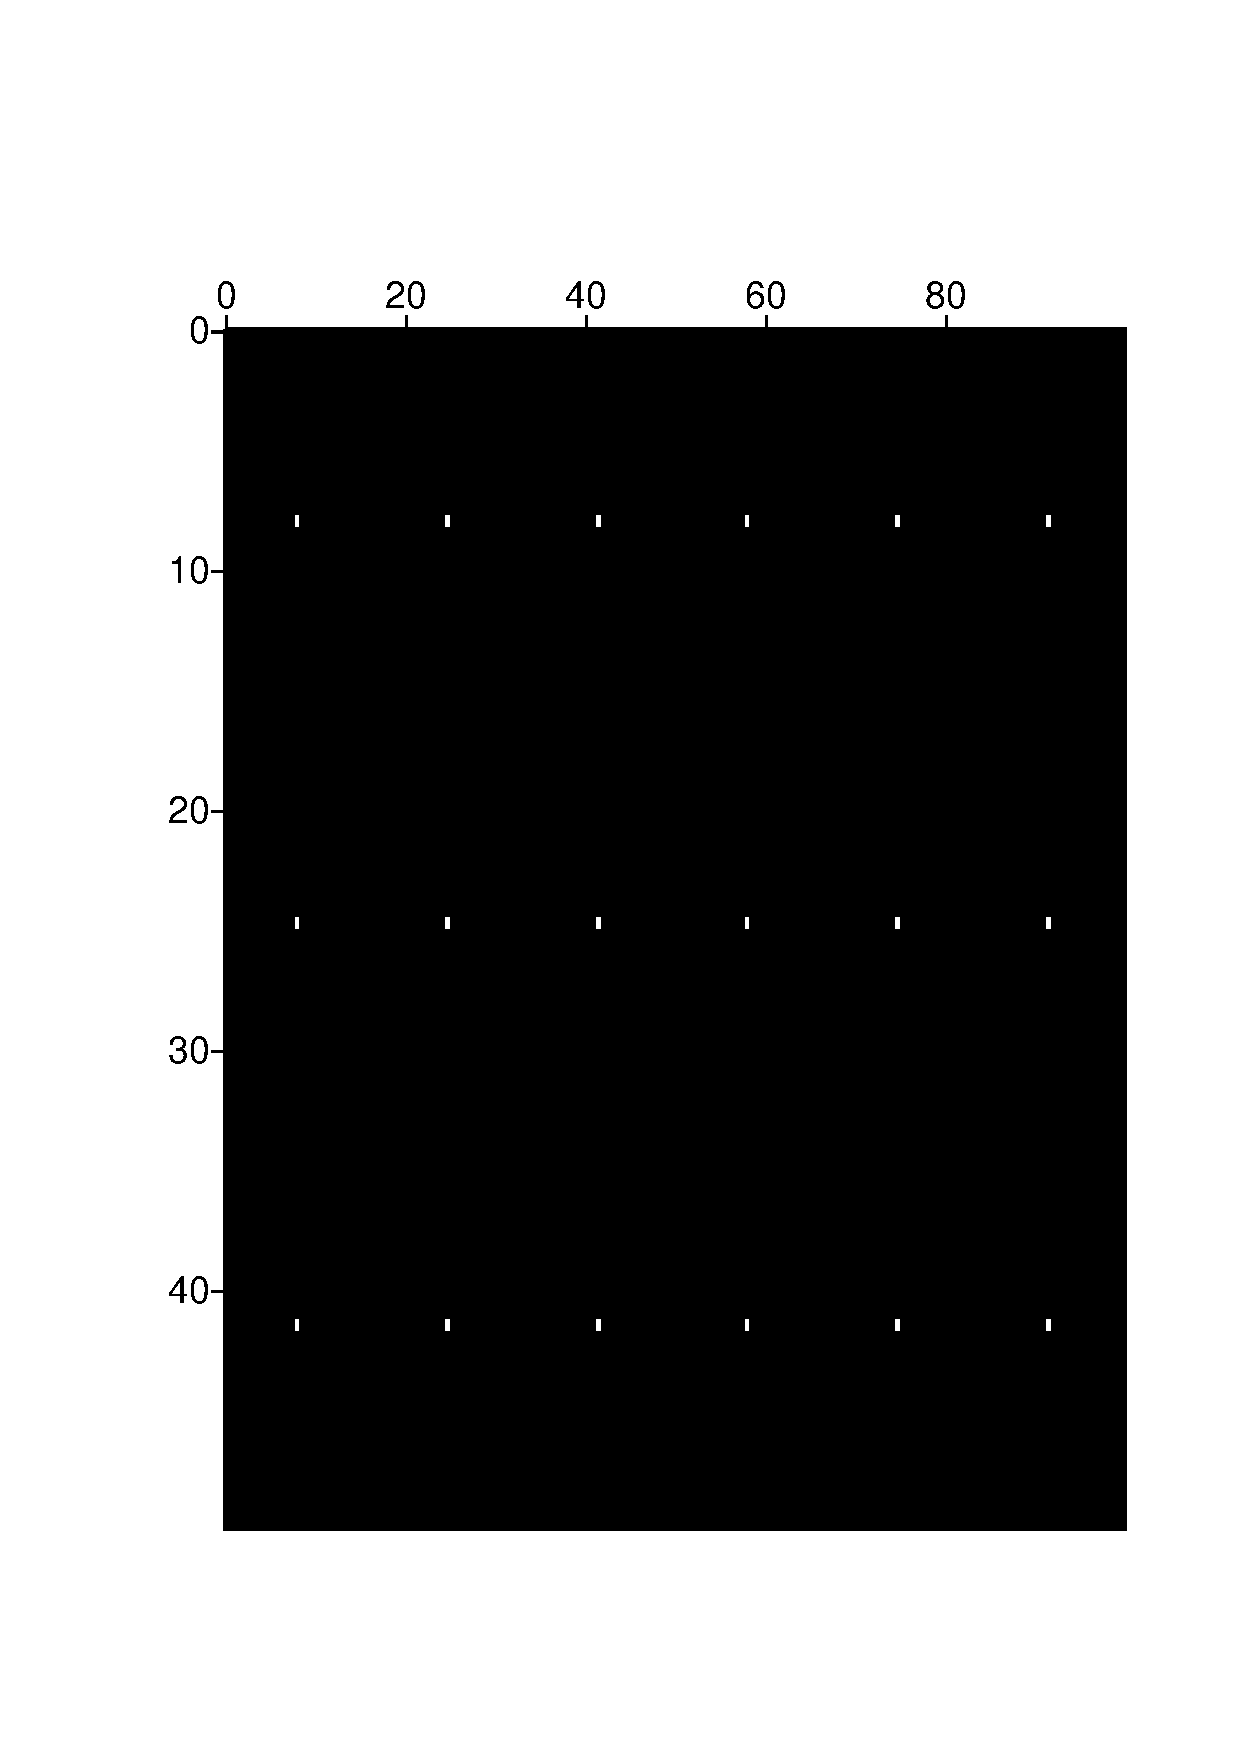
\includegraphics[height=5cm]{img/vp_scat.png}
	\caption{Configuration pour l'étude de résolution. La vitesse dans les inclusions est de 3000 m/s et de 6000 m/s ailleurs. \label{app:config_reso}}
\end{figure}

Le gradient est calculé en présence des dix-huit inclusions, sous l'hypothèse pour chaque inclusion, que la présence des autres n'intervient pas.\todo[inline]{à reformuler}

\subsection{Influence de la fréquence d'excitation}

Dans un premier temps, le milieu est entouré de conditions absorbantes. Les figures~\ref{app:150k} et~\ref{app:2M} montre la couverture en nombre d'onde obtenue dans une configuration avec une barrette excitatrice et pour deux gammes de fréquence différentes. 
    
\begin{figure}[!h]
    \centering
    \begin{subfigure}[b]{0.05\textwidth}
 		\hspace{-2cm}\includegraphics[width=0.5cm]{img/echelle_fft.png}\vspace{2.1cm}
	\end{subfigure}
    \begin{subfigure}[b]{0.4\textwidth}
		\hspace{-3cm}\includegraphics[width=1.5\textwidth]{img/ssfreesurf_150k}
		\caption{Excitation centrée à 150 kHz.}
		\label{app:150k}
	\end{subfigure}	
	%\hspace{0.7cm}
	\begin{subfigure}[b]{0.4\textwidth}
		\includegraphics[width=1.5\textwidth]{img/ssfreesurf_2M}
		\caption{Excitation centrée à 2 MHz.}
		\label{app:2M}
	\end{subfigure}
	\caption{Transformées de Fourier spatiales locales pour 2 gammes de fréquence d'excitation.}
\end{figure}

Dans le cas d'une excitation basse fréquence, le gradient est pauvre en hauts nombres d'onde. Inversement, l'excitation haute fréquence ne permet pas de reconstruire les bas nombres d'onde.\\
La couverture en nombre d'onde est également très liée à l'acquisition. Elle est meilleure aux abords et en direction de la barrette. Les nombres d'onde verticaux seront globalement mieux reconstruits avec cette acquisition, tandis que la couverture en nombres d'ondes horizontaux est très faible.

\subsection{Influence des surfaces libres}


\section{Gestion des non-linéarités}
Une stratégie pour limiter la non-linéarité de l'inversion consiste à réaliser l'inversion en plusieurs temps, en injectant progressivement le contenu haute fréquence dans les données. L'inversion à basse fréquence permet ainsi de reconstruire la structure grossière avant d'ajouter les détails grâce à la résolution qu'offre le gradient en haute fréquence.\\



Afin que les nombres imagés soient correctement échantillonnés, il faut que le plus grand nombre d'onde imagé à une fréquence soit le même que que le plus petit à la fréquence suivante \citep{sirgue}. En considérant que le plus nombre d'onde est obtenu pour une angle de diffraction de $\pi/2$ , le rapport de fréquences suivant doit donc être respecté : 

\begin{alignat*}{3}
	  ~&k_{max}(f_{n}) &&= k_{min}(f_{n+1})\\
	\Leftrightarrow~~~~~ &  f_n &&= f_{n+1}\cos \left(\frac{\pi}{2} \right)\\
	 \Leftrightarrow~~~~~ & \frac{f_{n+1}}{f_n} && \approx  1,5.
\end{alignat*} 

Les inversions présentées ci-après sont donc réalisées en plusieurs itérations. Entre chaque itérations, les données observées et l'ondelette d'excitation sont filtrées par un filtre passe-bas de fréquence centrale $f_{n}$ et dont la fréquence de coupure haute est de $2,5 \times f_{n}$.


\section{Équations de propagation pour le problème direct}

La propagation des ondes élastiques est décrite par les équations linéarisées en déplacements $\bm{u}$ et contraintes $\bar{\bar T}$ suivantes \citep{mat_ac} : 

\begin{eqnarray}
	\rho \frac{\dd^2 u_{i}}{\dd t^2} &=& \displaystyle\sum_{j}\frac{\dd T_{ij}}{\dd x_{j}}\\
	T_{ij}&=&C_{ijkl}\left( \frac{\dd u_{i}}{\dd x_{j}} + \frac{\dd u_{j}}{\dd x_{i}}\right)\text{,}
	\label{prop}
\end{eqnarray}
avec $C_{ijkl}$ le tenseur des constantes élastiques.

\subsection{Propagation acoustique}
Les équations de la propagation acoustique peuvent être déduite de~\ref{prop} en considérant un module de cisaillement nul. on a alors $T_{ij}=0$ si $i\neq j$.

\subsubsection{Isotrope}
Dans un milieu isotrope, les constantes élastiques sont égales dans toutes les directions. En milieu acoustique isotrope, les propriétés élastiques sont donc réduites à une seule constante et les équations~\ref{prop} deviennent : 
\begin{eqnarray}
	\rho \frac{\dd^2 u_{i}}{\dd t^2} = -\bm{\nabla} p\\
	p=-\kappa \displaystyle\sum_{i} \frac{\dd u_{i}}{\dd x_{i}}\text{,}
\end{eqnarray}
avec $\kappa$ le module de rigidité et $p$ la pression.

\subsubsection{Transverse isotrope}

Il est possible de formuler à partir de~\ref{prop} des équations d'ondes acoustiques en milieu anisotrope. Bien que ce soit physiquement impossible, cette formulation permet de se rapprocher cinématiquement des équations d'ondes élastiques, de manière simplifiée \citep{alkhalifah}.

Notons que cette formulation [Pose quelques problèmes (Duveneck 2008) notamment génération d'onde S (sur données "vrai simulée"  et sur problème direct, mais pas la même car différente grille, PML, ... donc on la mute sur le résidu) qui n'a pas de sens physique. Proposer les solutions (taper Epsilon, en sismo on est dans l'eau donc c'est fait naturellement -> placer les sources dans un milieu isotrope).]
 

La paramétrisation du milieu est faite à l'aide des constantes de Thomsen~\citep{thomsen} surtout utilisées dans le domaine des Sciences de la Terre définies comme suit : 
\begin{eqnarray}
	\epsilon & =  & \frac{C_{11}-C_{33}}{2C_{33}} = \frac{\bm{v}_{p}.\bm{e}_{x} -  \bm{v}_{p}.\bm{e}_{z}}{\bm{v}_{p}.\bm{e}_{z}}\\
	\delta & = & \frac{(C_{13}+C_{44})^2-(C_{33}-C_{44})^2}{2C_{33}(C_{33-C_{44}})}\text{.}\\
\end{eqnarray}
+theta

Le paramètre $\epsilon$ est donc lié à la différence entre la composante verticale et la composante horizontale de la vitesse des onde de pression et $\delta$ décrit davantage la propagation des ondes quasi-longitudinales.



\section{Inversions en matériau acoustique }

Dans un premier temps, la méthode d'imagerie est appliquée à des milieux acoustiques, ce qui simplifie le problème et réduit les coût de calcul. Les études proposées dans cette section sont menées en approximation 2D : on suppose que le problème ne dépend pas du tout de la dimension données par $\bm{e}_{y}$.\\

Le code utilisé est \emph{TOYxDacTIME} développé dans le cadre du projet \emph{Seiscope}\footnote{http://seiscope2.osug.fr}. Le problème direct y est résolu par différences finies, ce qui contraint 

\subsection{Isotrope}




monoparamètre : vp
multi paramètre ?



\subsection{VTI}
Afin d'introduire une anisotropie simplifiée dans la soudure, une étude dans un milieu acoustique VTI est menée.\\

On considère une plaque isotrope dans laquelle se trouve une soudure anisotrope VTI sans défaut. On cherche à évaluer l'influence de l'anisotropie en vue d'inverser le paramètre $\epsilon$. La valeur de $\epsilon$ dans la soudure est fixée à 20\%, ce qui est environ deux fois plus élevé que les valeurs que l'on peut trouver dans la littérature~\citep{chassignole}. Les deux barrettes excitatrices/réceptrices sont placées de manière éloignée, afin d'accentuer la propagation des ondes suivant $\bm{e}_{x}$ et de s'assurer que les temps de vol soient perturbés par l'anisotropie (figure~\ref{configuration_vti}).\\
Les autres paramètres ($v_{p}$,$\rho$ et $\delta$) sont supposés constants et uniformes.\\

Une comparaison des données observées en milieu isotrope ($\epsilon = 0$) et avec la soudure anisotrope est proposée en figure~\ref{}. Il apparaît que la présence d'une anisotropie VTI a peu d'impact sur les données, car le dispositif d'acquisition favorise la mesure des ondes dont le trajet est majoritairement vertical et donc peu perturbé.\\
 L'inversion du paramètre $\epsilon$ est alors difficile : une modification grossière de la vitesse horizontale suffit à corriger les retards résiduels (cf figure~\ref{}).
 
 \todo[inline]{figures : configurations ; traces isotrope, epsilon=20 ; inversion + données calculées}
 
Un modèle de soudure anisotrope VTI est donc trop simple pour représenter l'anisotropie d'une soudure réelle, dont on sait qu'elle impacte beaucoup le faisceau ultrasonore. Pour tester la capacité de la FWI à reconstruire ces paramètres d'anisotropie, il est donc nécessaire d'utiliser un modèle plus pertinent qui se rapprocherait davantage de celui proposé par \cite{ogilvy} par exemple.\\

Le modèle proposé par \cite{ogilvy} est de la forme : 
\begin{equation}
	\theta(x,z) = \tan^{-1}\left( \frac{D/2 + z\tan\alpha}{x} \right),
\end{equation}
avec $D$ la largeur de la racine de la soudure et $\alpha$  l'angle du bord de soudure.

 Conclusion : inversion de $\epsilon$ -> dur et par pertinent
passer en tilted (façon ogilvy ?) ou modèle plus précis en élastique.

\section{Inversions en matériau élastique isotrope}




%%%%%%%%%%%%%%%%%%%%%notes%%%%%%%%%%%%%%%
\todo[inline]{notes : }
\subsection{anisotrope}

anisotrope est plus problématique que isotrope car : 
-modélisation plus complexe,
-problème moins bien posé

Gholami 2011 : la vitesse a beaucoup plus d'influence sur les données que les paramètres delta et epsilon (delta étant le plus faible). D'après ses schémas, on va donc avoir une maj de la vitesse mais pas des autres paramètres

modèle initial de soudure : citer mina ?

%VTI elliptique ne gène pas l'inversion car beaucoup d'info portées par la transmission (vecteurs d'ondes verticaux non affectés par l'anisotropie elliptique VTI)  -> pas assez proche du modèle réel

%le flop du vti montre que l'inversion des paramètres est tributaire de l'acquisition

Romain : passer en TTI (code en freq)

